\begin{figure}[ht]
    \centering
    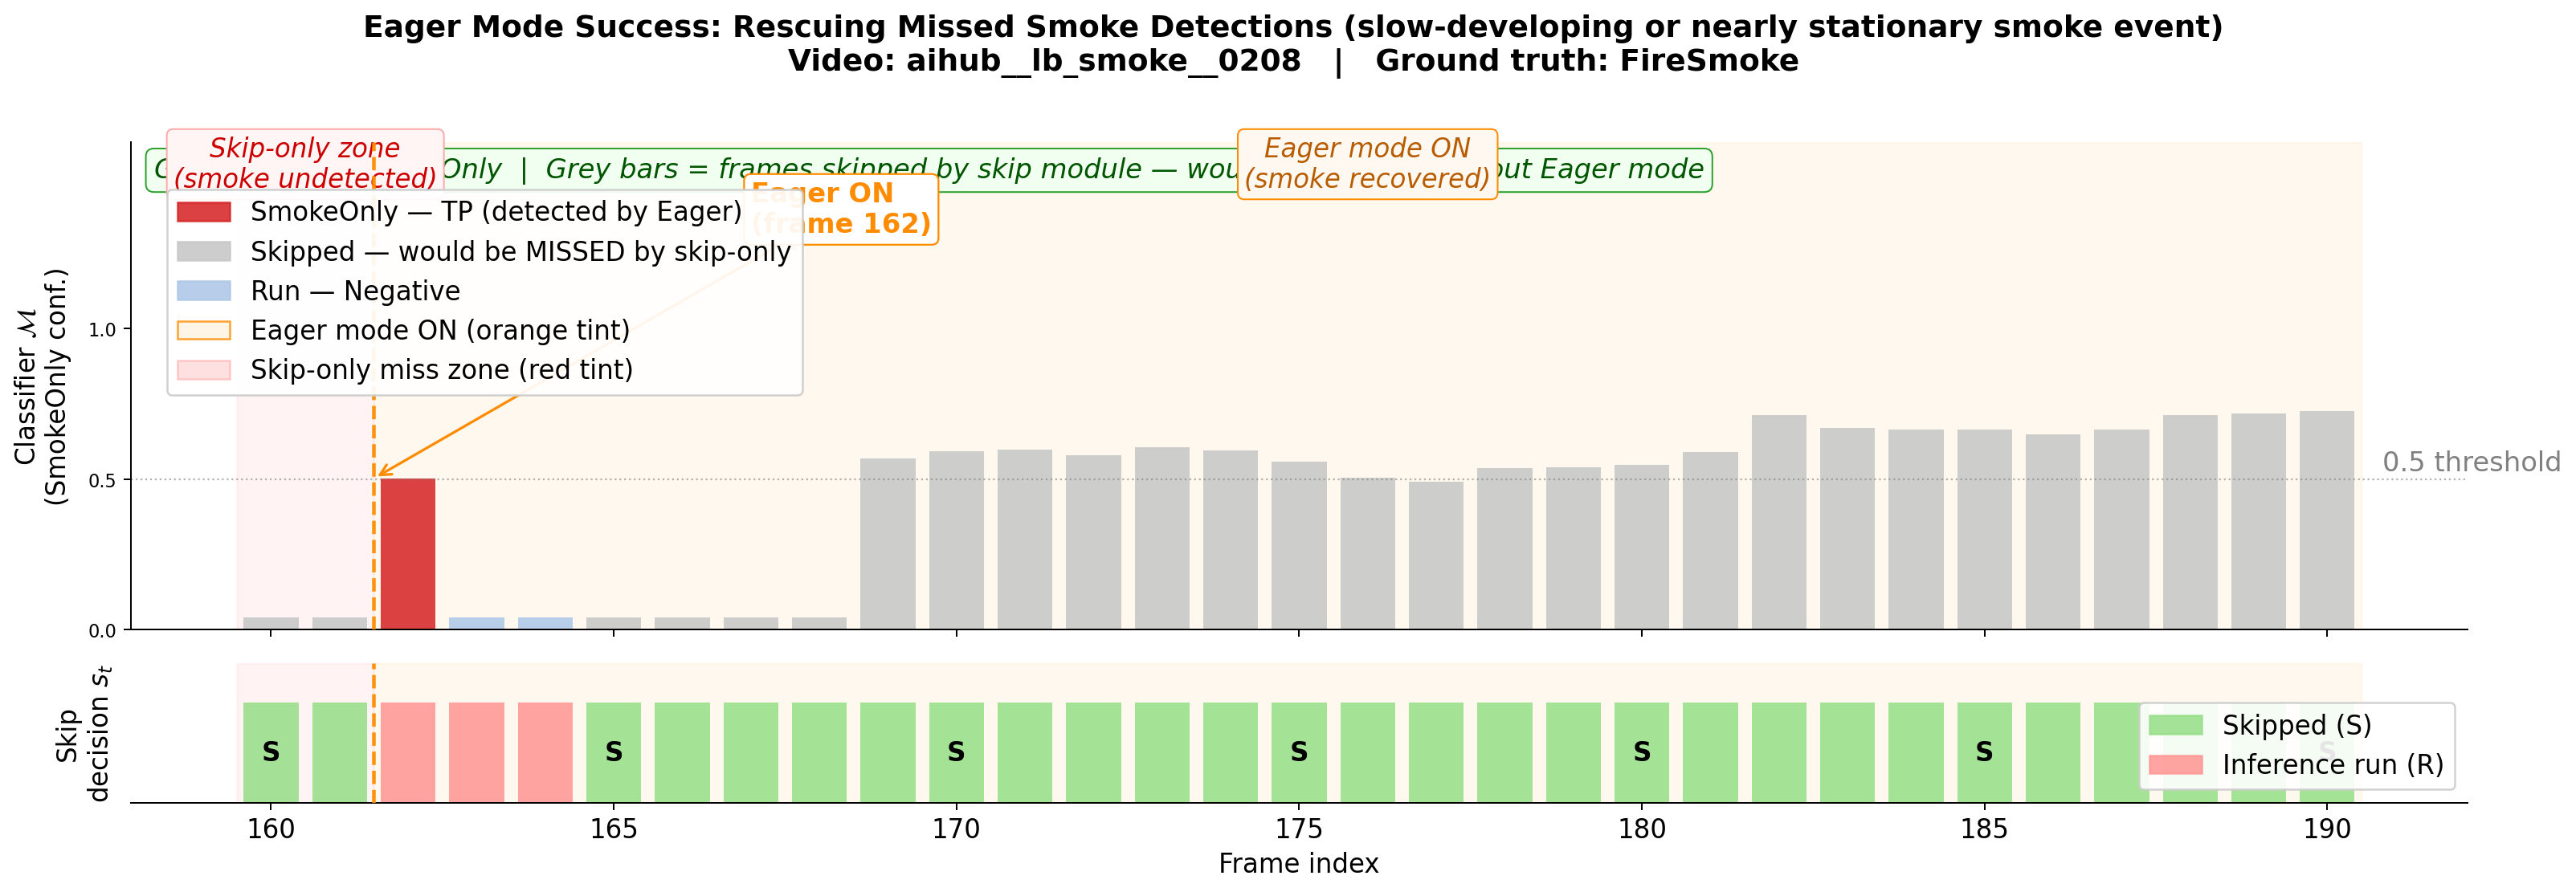
\includegraphics[width=\linewidth]{3.fig/eager_rs_analyse/eager_timeline_success.png}

    \caption{A per-frame timeline example illustrating a recall-recovery
        scenario under Eager mode. Initially, the skip module
        suppresses inference on
        slow-developing smoke frames with minimal inter-frame motion
        (Normal Mode Zone).
        Once the classifier $\mathcal{M}$ yields positive predictions on
        $W_{\text{fire}}=1$ consecutive frame(s) in Normal mode, the
        system transitions to
        Eager mode. This forces inference on every subsequent frame,
        enabling continuous
        smoke detection that would otherwise be missed---thus
        achieving a successful
        recall-recovery (\textcolor[HTML]{e8736f}{bars with light red}
        ). Notably, from frames 163 to 168, the system returns
        \texttt{None} predictions yet remains in Eager mode because
        the number of
        consecutive negative frames has not reached $W_{\text{clr}}=7$, which is
    insufficient to trigger an exit back to Normal mode.}
    \label{fig:eager_analysis_success}
\end{figure}
